\chapter{LND instrument}
\label{chp:LNDinstrument}

This supplement chapter provides the simulation setup of \ac{LND}, the overview of the \ac{LND} measurements in the last four years (2019 - 2023) and potential topics that worth to be investigated in the future.

\section*{LND simulation set-up}
\label{chp:LNDsimulation}

As explained by \citet{Wimmer-2020-LND}, response functions of the \ac{LND} to energetic particles are determined by the simulation using the \ac{Geant4} toolkit. In this section I explain the simulation setup of \ac{LND}.

Fig.~\ref{fig:LND_simulation_model} shows a screenshot of the \ac{LND} simulation model that we utilized. The model is a digital copy of the actual instrument, based on the computer-aided design (CAD) model, 
The outermost lines define the space where the simulation runs, which has a size of 20cm $\times$ 20cm $\times$ 20cm. The space inside the box is vacuum. The white structures in the middle is the housing of \ac{LND} sensor head, composed of Al boards.
The olive-colored layers in the sensor head are carriers of \acp{SSD} while \acp{SSD} are shown in blue color. The pink color indicated the location of Gd foils which are used to detect thermal neutrons. Next to the central detector stacks are two \acp{PCB} in green color.

\begin{figure}[!htb]
    \centering
    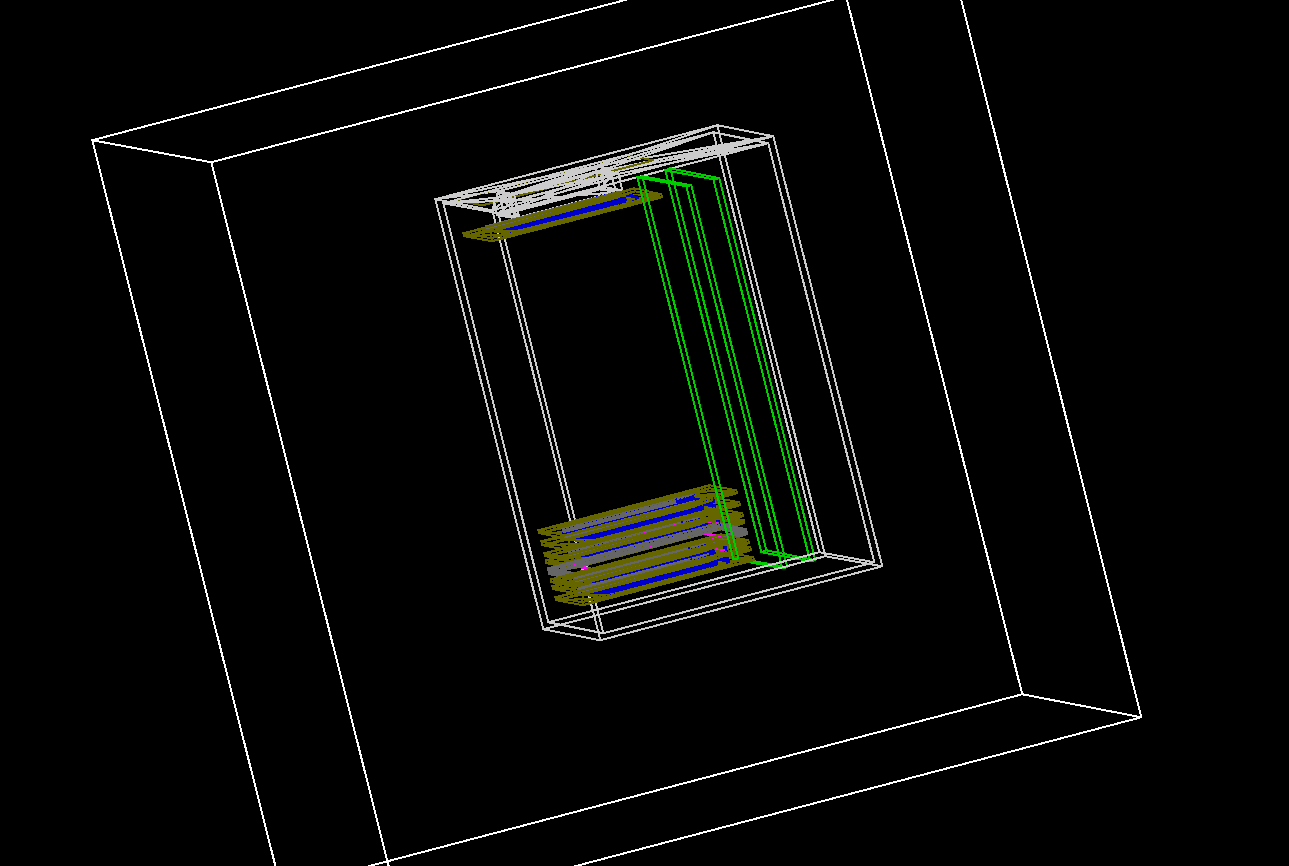
\includegraphics[width= 0.89\textwidth, height = 0.6\textwidth]{images/LND_model.png}
    \caption[The sketch of \ac{LND} sensor head]{The inner structure of the \ac{LND} sensor headthat is utilized in the \ac{Geant4} simultion. The sizes of each piece of structures are take from the CAD model of \ac{LND}}
    \label{fig:LND_simulation_model}
\end{figure}


\section*{The overall proton, helium and TID variation and the most updated SEP list}

\begin{figure}[!htb]
    \centering
    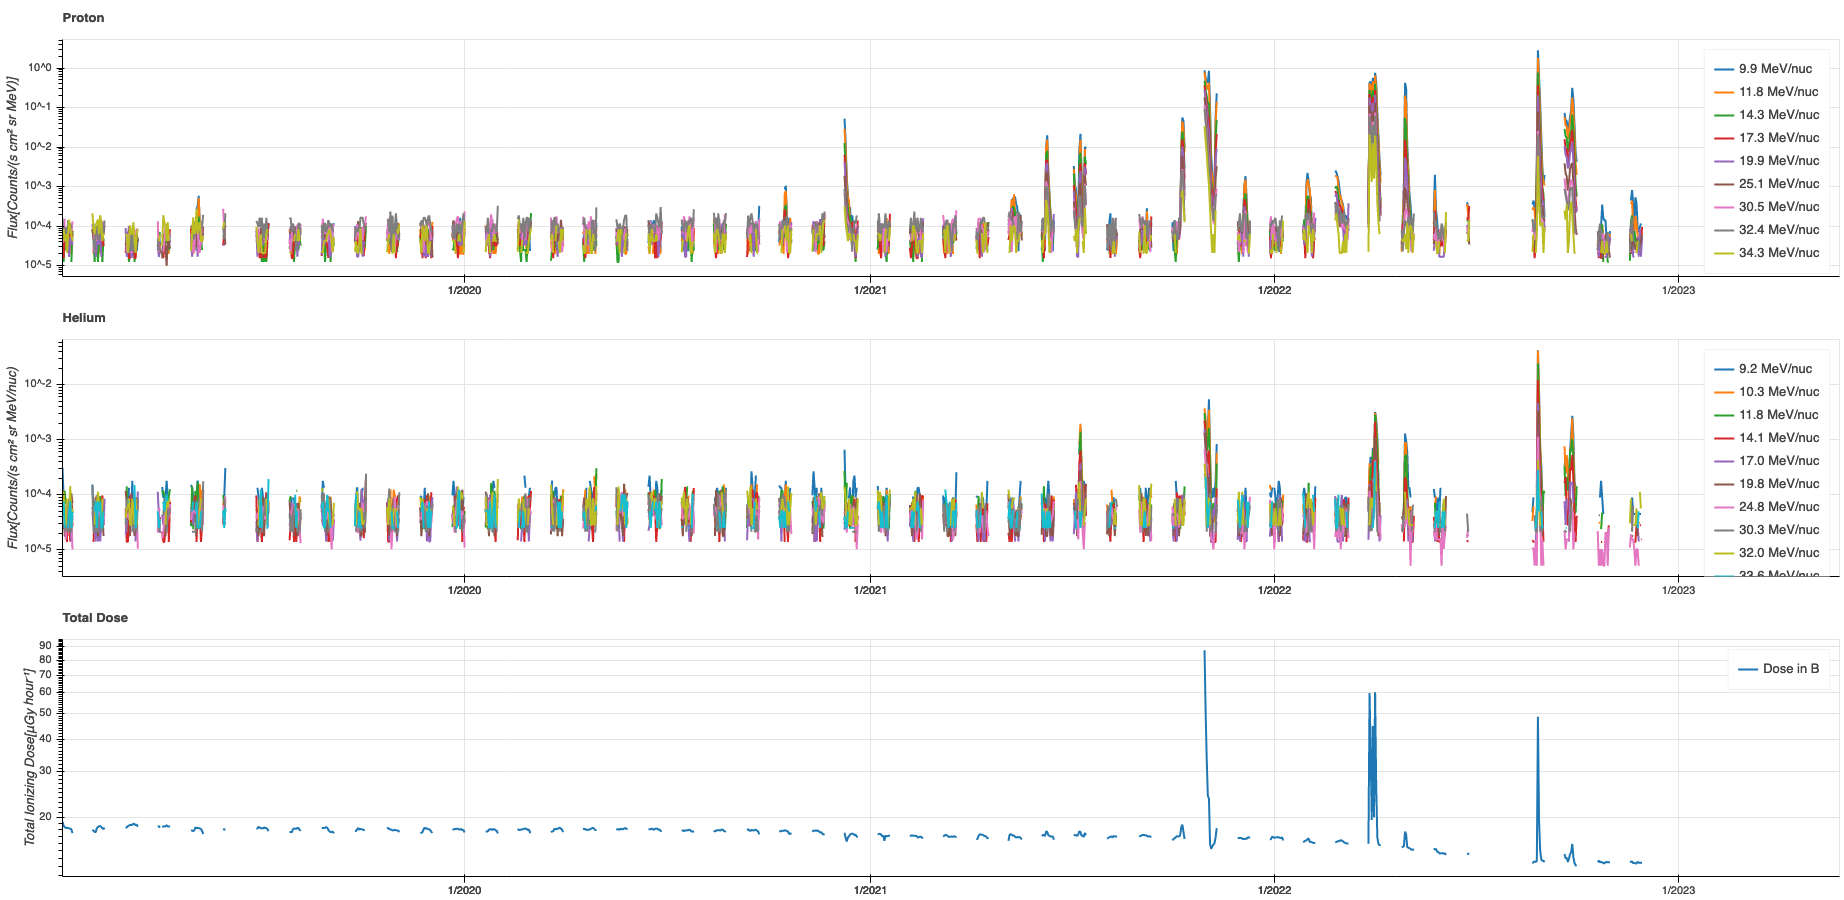
\includegraphics[angle = 90, width =\textwidth, height = 0.95\textheight]{images/LND-proton-helium-TID.png}
    \caption[The overview of proton, helium flux and \ac{TID} measured by \ac{LND}]{The proton, helium flux and \ac{TID} temporal variation from 2019 to Nov 29, 2022, measured by \ac{LND} on the lunar far-side surface}
    \label{Fig:appendix_LND_proton_helium_TID}
\end{figure}
\clearpage
Here we provide the overview of the proton, helium flux, and \ac{TID} temporal variation from 2019 to Nov 29, 2022, measured by \ac{LND} on the lunar far-side surface, as shown in Fig.~\ref{Fig:appendix_LND_proton_helium_TID}.
Figures are generated by the \ac{LND} webplotter, a web application used to visualize \ac{LND} data quickly. 
Currently, the webplotter is running on the server named etsasa and only be accessible to internal users.
The webplotter is written in Python, and the source codes are available in the GitHub repository \url{https://gitlab.physik.uni-kiel.de/LND/lnd_webplotter}.

The data gaps of \ac{LND} data appear periodically every lunar night. This gap is due to the switch off of instruments in order to survive during the lunar night. The more significant data gaps are periods when the lander conducts experiments. After 2021, more \ac{SEP} events are observed by \ac{LND}. Some of them even induced enhancement of \ac{TID} dramatically. 
It is worth noting that three consecutive \ac{SEP} events occurred in the April of 2022, as shown in Fig.~\ref{Fig:appendix_LND_proton_helium_TID}. The proton intensity increased after \ac{LND} switched on and returned back to the background level before the end of the lunar day. The completed proton, helium, and \ac{TID} time profiles are registered by \ac{LND}. Therefore, these three \ac{SEP} events provide an excellent opportunity to study the \acp{SEP} and its radiation impact on the lunar far-side surface.

In addition to the events that occurred on April 2022, other \ac{SEP} events are listed in table~\ref{Tab:appendix_LND_SEP_list}, including the first \ac{SEP} event in May 2019 and the first \ac{GLE} event at the end of 2021.

The start and end times of \ac{SEP} events are determined simply by eye inspection of proton time profiles. i.e. the top panel of Fig.~\ref{Fig:appendix_LND_proton_helium_TID}. If \ac{LND} did not register the complete time profile of \ac{SEP} events, the start time and end time of \ac{SEP} events are simply the starts and the end of the corresponding lunar day, respectively.
The letters Y/N in the radiation hazard column indicate whether this event causes an increase of \ac{TID}. The events of No.10, 15, and 18 are three \ac{SEP} events that cause a significant increase of \ac{TID} compared to others, and peak values of \ac{TID} are up to 50 $\mu Gy/hour$. The peak energy indicates the energy of the channel where the time profiles have clear enhancements.


% create a table of SEP list that LND measured
\begin{table}[!tbhp]
    \centering
    \caption[\acs{LND} \acs{SEP} events lists]{A list of \ac{SEP} events observed by \ac{LND} between 2019 and 2022}
\begin{tabular}{cccccc}
    \hline
    No.     &  Start time    & End time      & Radiation  & Peak energy \\
            &                &               & hazard      & (Proton, MeV)\\
    \hline
    1       &   2019-05-04 12:00 & 05-06 00:00               & N  & $\sim$ 10\\
    2       &   2019-05-06 06:00 & 05-06 18:00              & N  & $\sim$ 20 \\
    3       &   2019-10-16 18:00 & 10-19 00:00             & N  & $\sim$ 20 \\
    4       &   2019-12-09 06:00 & 12-12 00:00             & N  & $>$ 35 \\    
    5       &   2021-06-09 06:00 & 06-12 00:00             & Y  & $>$ 35 \\
    6       &   2021-07-04 06:00 & 07-07 00:00             & N  & $>$ 35 \\
    7       &   2021-07-09 10:00 & 07-12 06:00             & Y  & $>$ 35 \\
    8       &   2021-07-13 12:00 & 07-15 06:00             & Y  & $>$ 35 \\
    9       &   2021-10-09 06:00 & 10-12 00:00             & Y  & $>$ 35 \\
    10      &   2021-10-30 08:00 & 11-06 05:00             & Y(intense)  & $>$ 35\\
    11      &   2021-11-09 10:00 & 11-10 08:00             & Y  & $\sim$ 30 \\
    12      &   2021-12-05 05:00 & 12-07 09:00             & N  & $\sim$ 30 \\
    13      &   2022-01-29 22:00 & 02-03 11:00             & N  & $\sim$ 30 \\
    14      &   2022-02-25 06:00 & 03-01 19:00             & N  & $\sim$ 30 \\
    15(a,b,c) & 2022-03-28 06:00 & 04-07 01:00             & Y(intense)  & $>$ 35 \\
    16      &    2022-04-28 00:00 & 05-04 06:00             & Y  & $\sim$ 30 \\
    17      &   2022-05-25 16:00 & 05-26 23:00             & N  & $\sim$ 20\\
    18      &   2022-08-26 08:00 & 09-01 11:00             & Y(intense)  & $>$ 35 \\
    19      &   2022-09-19 23:00 & 09-39 00:00             & Y  & $\sim$ 30 \\
    20      &   2022-11-19 10:00 & 11-20 10:00             & N  & $\sim$ 15 \\
    \hline
\end{tabular}
\label{Tab:appendix_LND_SEP_list}
\end{table}



\section*{Housekeeping data of LND}

The instrument team use the housekeeping data of \ac{LND} check the current status and health of the instrument. Here, we present the temperature, bias current, and bias voltage.


\ac{LND} has six temperature sensors, monitoring the temperature variation of the \ac{SH} and the \ac{EB}. Two temperature sensors are placed near the \acp{SSD}, one inside of the \ac{EB}, and the remaining three are placed on the power board, the analog board, and the digital board. The time variations of temperature are given in panel (a) of Fig.\ref{Fig:appendix_LND_Housekeeping}. These sensors only measure in the daytime. The usual working temperature is above 20 degrees and has been increasing recently. The long-term seasonal temperature variation might be due to the change in the distance between the Moon and the Sun.

The other two housekeeping data we show are the bias current and bias voltage, which indicate the status of \acp{SSD}. Usually, the current is low, and the voltage is close to -150 V. The current and voltage variations are correlated with temperature, as the measurement of the first two lunar days shows.
However, as we explained in Section \ref{chp:instruments}, the particle signals of detectors A, H, I, and J are dominated by a massive amount of lower energy noise. Those noises cause the increase of bias current, reaching the upper limit of this channel, 2000 nA. Therefore, the bias voltage and bias current measurements are no longer reliable. We give the scripts that can be used to correct the bias voltage and bias current of \ac{LND} without any further explanation for documentary purposes. The scripts are from Stephan B\"{o}ttcher (private communication), the designer of \ac{LND}. Bias current $>$2000 nA is calculated from the bias voltage monitor by assuming a properly working power supply.



\begin{figure}[!htb]
    \centering
    \subfloat[]{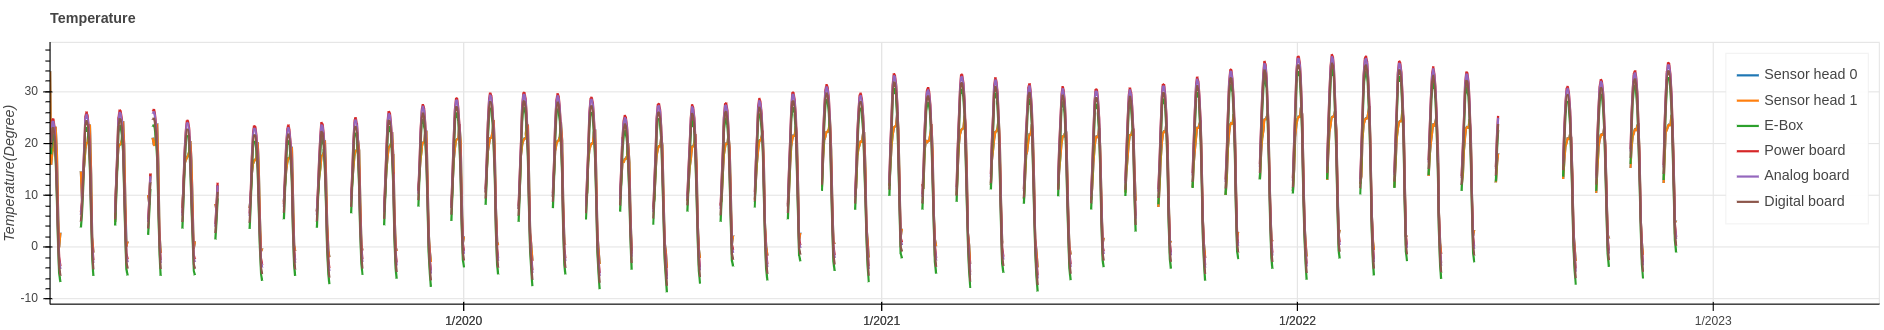
\includegraphics[angle =  90, width = 0.34\textwidth, height = 0.9\textheight]{images/lnd_temperature.png}}
    \subfloat[]{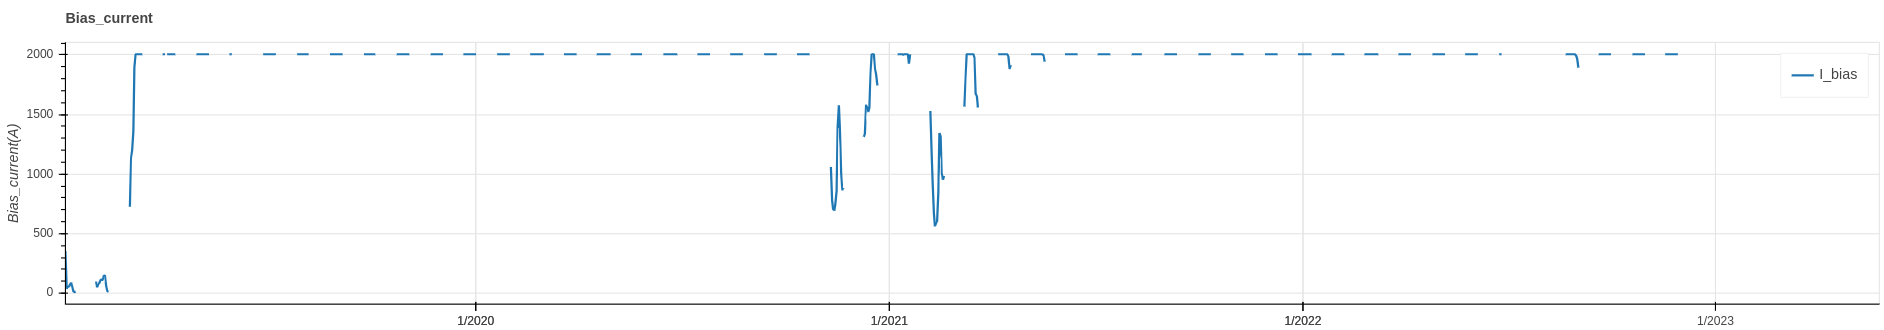
\includegraphics[angle = 90, width = 0.33\textwidth, height = 0.9\textheight]{images/lnd_bias_current.png}}
    \subfloat[]{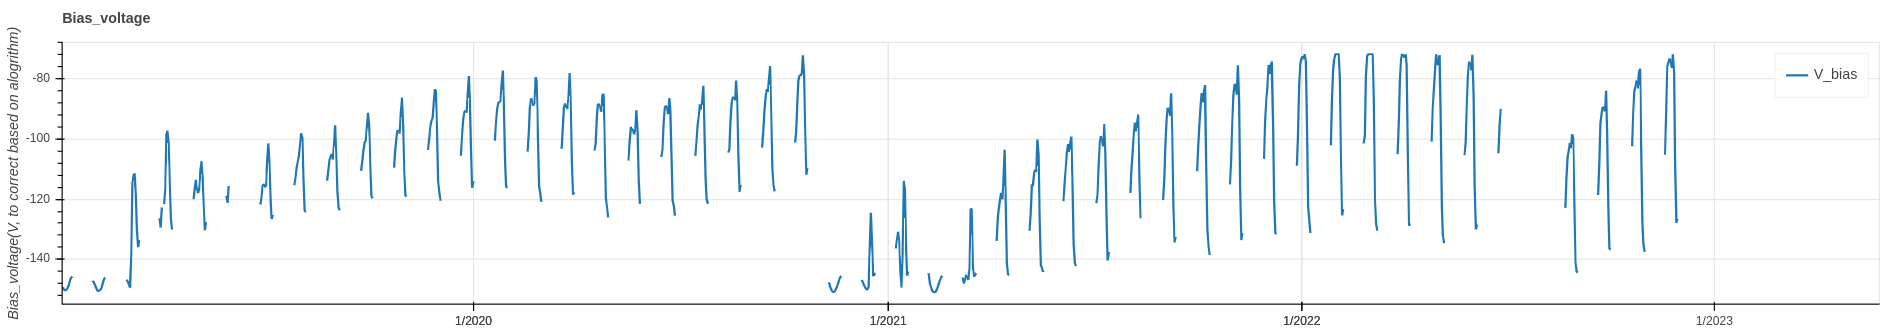
\includegraphics[angle = 90, width = 0.33\textwidth, height = 0.9\textheight]{images/lnd_bias_voltage.png}}
    \caption[LND temperature, bias current, and bias voltage variations]{The variation of housekeeping data including (a) temperature, (b) bias current, and (c) bias voltage. The temperatures are measured by the sensors assembled inside of LND sensor head and electronic box. The overview plot  2019 to Nov 29, 2022. }
    \label{Fig:appendix_LND_Housekeeping}
\end{figure}



\begin{lstlisting}[float]
# The Awk scripts for the LND bias current and voltage correction
# HK_Ibias and HK_Vbias are the bias current and voltage measured on the LND instrument
# LVPS represents low-voltage power supply of the LND instrument
# degC is the function to convert the temperature from Kelvin to Celsius
#================================
function Ibias() {
    a = $(HK_Ibias+3)
    if (a>4000) a = (147.3 + degC($(HK_T_LVPS+3))*0.164 - $(HK_Vbias+3)*0.05488) / 0.01810
    return a*0.4928
}
function Vbias() {
    return $(HK_Vbias+3)*0.05488 + $(HK_Ibias+3)*0.01810
}

\end{lstlisting}

\section*{Possible research topic related to LND data}
There still a lot 
The possible future work based on the \ac{LND} data includes:
\begin{itemize}

    \item Heavy ion measurements of \ac{LND}: The heavy ions are an important component of \ac{LND} data products. Currently, the published data products count the C, N, and O in one channel and heavier ions in one channel. We can derive and create the data products of different particle species with further calibration and data analysis.
    \item Studying the discrepancy of \ac{TID} between \ac{LND} and \ac{CRaTER}: In \citet{Zhang2020SciAdv}, we have shown that the dose rate measured in two instruments are consistent during the first two lunar days. However, my preliminary results from comparing two years' data showed that the long-term variation of \ac{TID} and \ac{CRaTER} have different tendencies and are not consistent in the long run. This is out of our expectations. The possible reasons include the decay of the neutral source of \ac{LND} and the different responses of the two instruments.
    \item Albedo proton spectrum with better energy resolution: Currently, due to the counting statistic considerations, we only define albedo protons between 65 - 76 MeV as a single data point. In the future, with more than four years of data collection, data products of refined energy resolution will also be possible. Furthermore, two dimensions \ac{LET} measurement could also be used to study the albedo particles and potentially derive the dose rate of albedo particles.
    \item $^3$He measured by \ac{LND}: The reliable $^3$He data products of \ac{LND} should be generated, and the $^3$He/$^4$He ratio in the energy range of 10 - 35 MeV/nuc should be derived.
    \item Instrument responce of \ac{TID} to \acp{SEP}: The \ac{TID} could be predicted by assuming an input spectra. The analysis could help understand the instrument and relationship between \ac{SEP} and \ac{TID}.
    \item Jovian electrons.



\end{itemize}

% \subsection*{}


% \subsection{He3 spectra}
% \label{chp:appendix_LND_He3_spectra}
% Mostly the instrument effect, the He3 spectra is not reliable.


% \section{Responce of TID to SEPs}
% and provide invaluable insight into our heliosphere. 
% Though \ac{LND} have been troubled by the noise issue and discoutinuity of the data due to the special working environment on the lunar suface, the large amount of \ac{LND} data have large potential in contributing to our understanding of the inteaction between charged particle and environement. One of the interesting topic is linking \ac{TID} measurements with energetic particles measurements. In order to achive this, we first need to derive the response of \ac{LND} to the charged particle with power law input spectra. Then we fold different input spectra with the response function to predict the possible \ac{TID} on the lunar surface. Finally, we compare the predicted \ac{TID} with the measured \ac{TID} to validate the current model. By doing so, we could have better understanding of the instrument itself and the radiation environment on the lunar surface.
